\documentclass[10pt]{beamer}

\usetheme[progressbar=frametitle]{metropolis}
\usepackage{appendixnumberbeamer}
\usepackage{multicol}
\usepackage{hyperref}
\usepackage{listings}
\usepackage{color}
\usepackage{tikz}
\usepackage[utf8]{inputenc}

\newcommand{\themename}{\textbf{\textsc{metropolis}}\xspace}


\DeclareFixedFont{\ttb}{T1}{txtt}{bx}{n}{12}
\DeclareFixedFont{\ttm}{T1}{txtt}{m}{n}{12}

\definecolor{codegreen}{rgb}{0,0.6,0}
\definecolor{codegray}{rgb}{0.5,0.5,0.5}
\definecolor{codepurple}{rgb}{0.58,0,0.82}
\definecolor{backcolour}{rgb}{0.95,0.95,0.9}
\definecolor{deepblue}{rgb}{0,0,0.5}
\definecolor{deepred}{rgb}{0.6,0,0}
\definecolor{deepgreen}{rgb}{0,0.5,0}
\definecolor{uislight}{HTML}{0a3c9f}
\definecolor{uisdark}{HTML}{0a3ca0}
\definecolor{uisorange}{HTML}{ff9e3d}
\definecolor{uisgrey}{HTML}{e1e1e1}

\lstdefinestyle{mystyle}{
    language=Python,
    basicstyle=\ttfamily\tiny,
    morekeywords={self},
    keywordstyle=\ttb\color{deepblue},
    emph={MyClass,__init__},
    emphstyle=\ttb\color{deepred},
    stringstyle=\color{deepgreen},
    frame=tb,
    showstringspaces=false
    commentstyle=\color{codegreen},
    keywordstyle=\color{magenta},
    numberstyle=\tiny\color{codegray},
    stringstyle=\color{codepurple},
    breakatwhitespace=false,         
    breaklines=true,                 
    captionpos=b,                    
    keepspaces=true,                 
    numbers=left,                    
    numbersep=5pt,                  
    showspaces=false,                
    showstringspaces=false,
    showtabs=false,                  
    tabsize=2
}

\lstset{style=mystyle}


\setbeamercolor{palette primary}{bg=uisdark,fg=white}
\setbeamercolor{frametitle}{bg=uislight}
\setbeamercolor{progress bar}{fg=uisorange, bg=uisgrey}

\makeatletter
\setlength{\metropolis@titleseparator@linewidth}{1pt}
\setlength{\metropolis@progressonsectionpage@linewidth}{1pt}
\setlength{\metropolis@progressinheadfoot@linewidth}{1pt}
\makeatother


\title{Finding Flight Delay Trends}
\subtitle{DAT500 Project Group 17}
% \date{\today}
\date{}
\author{Bhakti Prabhu \& Stephan F. W. Brandasu}
\institute{Faculty of Science and Technology}

\titlegraphic{\hfill
\includegraphics[height=2cm]{images/logo.png}}

\begin{document}

\maketitle


\begin{frame}{Why \& What\\ \small the use case}
\begin{multicols}{2}
As a traveller: 
\begin{enumerate}
    \item Not miss any important meetings/events/functions.
    \item Pre-plan journey
    \item Have idea of buffer time while flight booking
\end{enumerate}
As an airline:
\begin{enumerate}
    \item  know when to increase workforce.
    \item Opportunity to improve over competitors.
\end{enumerate}
\columnbreak
Objective:
\begin{enumerate}
    \item visualise delay trends over time
    \item how well do the airlines catch up when departing late
    \item how often are flights cancelled
    \item are longer flights delayed more often
\end{enumerate}
\end{multicols}
\end{frame}


\begin{frame}{The Dataset}
From 20GB of unstructured .txt files to 6GB of .csv
\begin{multicols}{2}
\begin{figure}
    \centering
    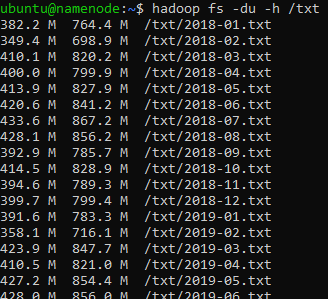
\includegraphics[width=5cm]{images/unstructured_dataset_size.png}
    \label{fig:unstructured}
\end{figure}
\columnbreak
\begin{figure}
    \centering
    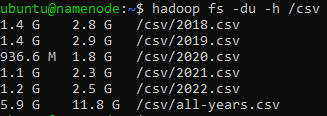
\includegraphics[width=5cm]{images/structured_dataset_size.png}
    \label{fig:structured}
\end{figure}
\end{multicols}
\end{frame}


\begin{frame}{The Dataset}
\tiny{}
\usetikzlibrary{decorations.pathreplacing,shapes,arrows,positioning}
\usetikzlibrary{calc}
\usetikzlibrary{shapes.geometric, arrows}


\definecolor{mycolor1}{RGB}{0, 0, 128} % Navy
\definecolor{mycolor2}{RGB}{30, 144, 255} % Dodger Blue
\definecolor{mycolor3}{RGB}{34, 139, 34} % Forest Green
\definecolor{mycolor4}{RGB}{255, 165, 0} % Orange
\definecolor{mycolor5}{RGB}{218, 112, 214} % Orchid
\definecolor{mycolor6}{RGB}{255, 0, 255} % Magenta
\definecolor{mycolor7}{RGB}{128, 0, 0} % Maroon
\definecolor{mycolor8}{RGB}{255, 192, 203} % Pink
\definecolor{mycolor9}{RGB}{46, 139, 87} % Sea Green
\definecolor{mycolor10}{RGB}{255, 99, 71} % Tomato
\definecolor{mycolor11}{RGB}{128, 128, 128} % Gray


\tikzstyle{arrow} = [line width=0.10mm,->,shorten >=8pt, shorten <=2pt]

\begin{tikzpicture}[node distance=0.21cm and 3.5cm]
\tikzstyle{every node}=[font=\ttfamily\tiny]

\node (a1)[text=mycolor1]{year};
\node (a2)[below of=a1] {quarter};
\node (a3)[below of=a2, text=mycolor2] {month};
\node (a4)[below of=a3] {day\_of\_month};
\node (a5)[below of=a4] {day\_of\_week};
\node (a6)[below of=a5, text=mycolor3] {fl\_date};
\node (a7)[below of=a6, text=mycolor4] {op\_unique\_carrier};
\node (a8)[below of=a7] {tail\_num};
\node (a9)[below of=a8] {op\_carrier\_fl\_num};
\node (a10)[below of=a9, text=mycolor5] {origin\_airport\_id};
\node (a11)[below of=a10] {origin\_airport\_seq\_id};
\node (a12)[below of=a11] {origin\_city\_market\_id};
\node (a13)[below of=a12] {origin};
\node (a14)[below of=a13] {origin\_city\_name};
\node (a15)[below of=a14] {origin\_state\_nm};
\node (a16)[below of=a15, text=mycolor6] {dest\_airport\_id};
\node (a17)[below of=a16] {dest\_airport\_seq\_id};
\node (a18)[below of=a17] {dest\_city\_market\_id};
\node (a19)[below of=a18] {dest};
\node (a20)[below of=a19] {dest\_city\_name};
\node (a21)[below of=a20] {dest\_state\_nm};
\node (a22)[below of=a21] {dep\_delay};
\node (a23)[below of=a22, text=mycolor7] {dep\_delay\_new};
\node (a24)[below of=a23] {dep\_del15};
\node (a25)[below of=a24] {arr\_delay};
\node (a26)[below of=a25, text=mycolor8] {arr\_delay\_new};
\node (a27)[below of=a26] {arr\_del15};
\node (a28)[below of=a27, text=mycolor9] {cancelled};
\node (a29)[below of=a28] {cancellation\_code};
\node (a30)[below of=a29, text=mycolor10] {diverted};
\node (a31)[below of=a30, text=mycolor11] {air\_time};
\node (a32)[below of=a31] {distance};
\node (a33)[below of=a32] {distance\_group};
\node (a34)[below of=a33] {carrier\_delay};
\node (a35)[below of=a34] {weather\_delay};
\node (a36)[below of=a35] {nas\_delay};
\node (a37)[below of=a36] {security\_delay};
\node (a38)[below of=a37] {late\_aircraft\_delay};


\node (b1)[right =of a1, text=mycolor1]{year};
\node (b2)[below of= b1, text=mycolor2] {month};
\node (b3)[below of= b2, text=mycolor3] {fl\_date};
\node (b4)[below of= b3, text=mycolor4] {op\_unique\_carrier};
\node (b5)[below of= b4, text=mycolor5] {origin\_airport\_id};
\node (b6)[below of= b5, text=mycolor6] {dest\_airport\_id};
\node (b7)[below of= b6, text=mycolor7] {dep\_delay\_new};
\node (b8)[below of= b7, text=mycolor8] {arr\_delay\_new};
\node (b9)[below of= b8, text=mycolor9] {cancelled};
\node (b10)[below of= b9, text=mycolor10] {diverted};
\node (b11)[below of= b10, text=mycolor11] {air\_time};


\node (c1)[right =of b1, text=mycolor1]{year};
\node (c2)[below of= c1, text=mycolor2] {month};
\node (c3)[below of= c2, text=mycolor4] {op\_unique\_carrier};
\node (c4)[below of= c3, text=mycolor5] {origin\_airport\_id};
\node (c5)[below of= c4, text=mycolor6] {dest\_airport\_id};
\node (c6)[below of= c5, text=mycolor8] {max\_arr\_delay};
\node (c7)[below of= c6, text=mycolor3] {max\_arr\_delay\_fl\_date};
\node (c8)[below of= c7, text=mycolor8] {avg\_arr\_delay};
\node (c9)[below of= c8, text=mycolor8] {med\_arr\_delay};
\node (c10)[below of= c9, text=mycolor6] {avg\_time\_recovered};
\node (c11)[below of= c10, text=mycolor10] {nr\_diverted};
\node (c12)[below of= c11, text=mycolor11] {avg\_airtime};
\node (c13)[below of= c12] {flight\_count};
\node (c14)[below of= c13, text=mycolor9] {nr\_cancelled};



\end{tikzpicture}
\end{frame}


\begin{frame}[fragile]{Mapping}
\begin{multicols}{2}
\begin{lstlisting}
import sys

row = []

for line in sys.stdin:
  line = line.strip().replace(',','').split()

  if line[0] == "LATE_AIRCRAFT_DELAY":
    try:
      data = line[1]
    except IndexError:
      data = ' '
    row.append(data)
    print(','.join(row))
    row = []
  else:
    try:
      data = ' '.join(line[1:])
    except IndexError:
      data = ' '
    row.append(data)
\end{lstlisting}
\columnbreak
\begin{itemize}
    \item create array of each row
    \item remove any unwanted commas from cell
    \item check for last column of row
    \item catch error in case of no data in current column
    \item print row
\end{itemize}
\end{multicols}
\end{frame}


\begin{frame}[fragile]{Reading the data}
\begin{multicols}{2}
\begin{lstlisting}
flight_data = spark.read.csv('hdfs://namenode:9000/csv/'+sys.argv[1]+'.csv', schema=flightSchema)\
.withColumn('FL_DATE', to_date(to_timestamp('FL_DATE', 'M/d/yyyy h:mm:ss a')))

flight_data = flight_data.select( 'year'
                        , 'month'
                        , 'fl_date'
                        , 'op_unique_carrier'
                        , 'origin_airport_id'
                        , 'dest_airport_id'
                        , 'dep_delay_new'
                        , 'arr_delay_new'
                        , 'cancelled'
                        , 'diverted'
                        , 'air_time')

flight_data = flight_data.na.drop(subset=['year', 'origin_airport_id', 'dest_airport_id', 'fl_date'])
flight_data = flight_data.fillna({'arr_delay_new': 0.0})
\end{lstlisting}
\columnbreak
\begin{itemize}
    \item select only relevant columns
    \item drop any rows that are missing essential information
    \item fill 0.0 in rows to avoid issues during calculations
\end{itemize}
\end{multicols}
\end{frame}


\begin{frame}[fragile]{Manipulating the data - step 1}
\begin{multicols}{2}
\begin{lstlisting}
# grab the fl_date of the flight with the highest delay for a given group
windowSpec = Window.partitionBy(
      'year'
    , 'month'
    , 'op_unique_carrier'
    , 'origin_airport_id'
    , 'dest_airport_id').orderBy(col('arr_delay_new').desc())
    
arr_delay_dates = flight_data.withColumn(
        'rank'
    , rank().over(windowSpec)
).filter(
    col('rank') == 1
).groupBy(
      'year'
    , 'month'
    , 'op_unique_carrier'
    , 'origin_airport_id'
    , 'dest_airport_id'
).agg(
round(max('arr_delay_new'), 2).alias('max_arr_delay')
, first('fl_date').alias('max_arr_delay_fl_date')
)
\end{lstlisting}
\columnbreak
\begin{itemize}
    \item create a window sorted by the arrival delay
    \item select the top delay date by only selecting single row
\end{itemize}
\end{multicols}
\end{frame}


\begin{frame}[fragile]{Manipulating the data - step 2}
\begin{multicols}{2}
\begin{lstlisting}
flight_data = flight_data.groupBy('year'
, 'month'
, 'op_unique_carrier'
, 'origin_airport_id'
, 'dest_airport_id').agg( round(avg('arr_delay_new'), 2).alias('avg_arr_delay')
    , round(percentile_approx('arr_delay_new', 0.5), 2).alias('med_arr_delay')
    , round(avg(col('dep_delay_new') - col('arr_delay_new')), 2).alias('avg_time_recovered')
    , sum('diverted').alias('nr_diverted')
    , round(avg('air_time'), 2).alias('avg_airtime')
    , count('*').alias('flight_count')
    , sum('cancelled').alias('nr_cancelled'))

flight_data = arr_delay_dates.join( flight_data
    , on=['year', 'month', 'op_unique_carrier', 'origin_airport_id', 'dest_airport_id']
    , how='left')
\end{lstlisting}
\columnbreak
\begin{itemize}
    \item do a groupby select for to grab delay statistics
    \item each result is rounded to 2 decimals to avoid ugly numbers
    \item join the result of this operation with the previous one
\end{itemize}
\end{multicols}
\end{frame}


\begin{frame}[fragile]{Upserting into the DeltaTable}
\begin{lstlisting}
# Checking if Table exists
if DeltaTable.isDeltaTable(spark, "hdfs://namenode:9000/spark-warehouse/sample_flight_table"):
    # Perform the upsert operation
    deltaDF = DeltaTable.forPath(spark, "hdfs://namenode:9000/spark-warehouse/sample_flight_table")
    merge_condition = "existing.year = upsert.year \
    AND existing.month = upsert.month \
    AND existing.op_unique_carrier = upsert.op_unique_carrier \
    AND existing.origin_airport_id = upsert.origin_airport_id \
    AND existing.dest_airport_id = upsert.dest_airport_id "

    deltaDF.alias('existing') \
        .merge(flight_data.alias('upsert'), merge_condition) \
        .whenMatchedUpdateAll() \
        .whenNotMatchedInsertAll() \
        .execute()  
else:
    # Create new delta table
    flight_data.write.format("delta").mode("overwrite").saveAsTable("sample_flight_table")
\end{lstlisting}

\end{frame}




\begin{frame}[fragile]{Skew \& Spill}
\begin{multicols}{2}

Optmization (spark-defaults.conf)
\begin{lstlisting}
spark.executor.memory                   6g
spark.exector.instances                 3
spark.executor.cores                    4
spark.sql.shuffle.partition             64
spark.sql.adaptive.skewedJoin.enabled   true
spark.sql.adaptive.skewJoin.enabled     true
\end{lstlisting}

\columnbreak
\begin{table}[]
    \centering
    \begin{tabular}{c|c|c}
        \textbf{Spill} & \textbf{Memory} & \textbf{Disk} \\
        \hline 
        \textbf{Before} & 3.5 GiB & 177.8 MiB \\
        \hline
        \textbf{After} & 128.4 MiB & 7.1 MiB 
        \end{tabular}
    \label{tab:spill}
\end{table}

\begin{figure}
    \centering
    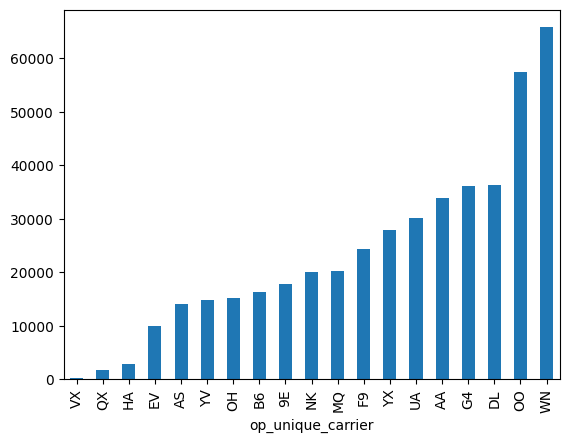
\includegraphics[width=5cm]{images/skew.png}
    \label{fig:skew}
\end{figure}
\end{multicols}
\end{frame}




\begin{frame}[fragile]{Serialization}
\begin{multicols}{2}
Using UDF's to clean the data
\begin{lstlisting}
def replace_null(value, default):
  if value is None:
    return default
  return value

def drop_null(*cols):
  for col in cols:
    if col is None:
      return False
  return True

replace_null_udf = udf(lambda value, default: replace_null(value, default), FloatType())
drop_null_udf = udf(lambda *cols: drop_null(*cols), BooleanType())

flight_data = flight_data.filter(drop_null_udf(*[col(c) for c in ['year', 'origin_airport_id', 'dest_airport_id', 'fl_date']]))
flight_data = flight_data.withColumn('arr_delay_new', replace_null_udf(col('arr_delay_new'), lit(0.0)))
\end{lstlisting}
\columnbreak
Performance difference between each type of join
\begin{table}[]
    \centering
    \begin{tabular}{c|c|c}
      & \textbf{normal} & \textbf{udf} \\
      \hline
     \textbf{minutes} & 2.8  & 7.1
    \end{tabular}
    \label{tab:udf}
\end{table}

\end{multicols}
\end{frame}


\begin{frame}[fragile]{Shuffle}
\begin{multicols}{2}
sort merge join
\begin{lstlisting}
arr_delay_dates = arr_delay_dates.sort(['year', 'month', 'op_unique_carrier', 'origin_airport_id', 'dest_airport_id'])
flight_data = flight_data.sort(['year', 'month', 'op_unique_carrier', 'origin_airport_id', 'dest_airport_id'])

# join the highest delay with the res of the group
flight_data = arr_delay_dates.join( flight_data
, on=['year', 'month', 'op_unique_carrier', 'origin_airport_id', 'dest_airport_id']
, how='left')
\end{lstlisting}
\columnbreak
broadcast join
\begin{lstlisting}
flight_data = arr_delay_dates.join( 
    broadcast(flight_data)
    , on=['year', 'month', 'op_unique_carrier', 'origin_airport_id', 'dest_airport_id']
    , how='left')
\end{lstlisting}
\begin{table}[]
    \centering
    \begin{tabular}{c|c|c}
      & \textbf{Sort Merge} & \textbf{Broadcast} \\
      \hline
     \textbf{Minutes} & 4.1  & 3.2
    \end{tabular}
    \label{tab:join}
\end{table}
\end{multicols}
\end{frame}



\begin{frame}[fragile]{Graphs from the delta table}

\begin{lstlisting}
builder = SparkSession.builder.appName('flight_plot')
spark = configure_spark_with_delta_pip(builder).getOrCreate()

flight_data = spark.read.format('delta').load('hdfs://namenode:9000/spark-warehouse/flight_data_table')

flight_data = flight_data.filter((flight_data.op_unique_carrier == 'AA') & (flight_data.origin_airport_id == 12892) & (flight_data.dest_airport_id == 12478))

flight_data = flight_data.orderBy('year', 'month')

flight_data = flight_data.withColumn('year_month', concat('year', lit('-'), 'month'))

flight_data = flight_data.toPandas()

avgdelay = normalize(flight_data, "avg_arr_delay")
flightcount = normalize(flight_data, "flight_count")

data = [
plt.Scatter(x=flight_data.year_month
            , y=avgdelay
            , name='average flight delay over time'
            , text=flight_data.avg_arr_delay),
plt.Scatter(x=flight_data.year_month
            , y=flightcount
            , name='nr of flights'
            , text=flight_data.flight_count),
]

fig = plt.Figure(data, layout_title_text='delay over time with nr of flights normalized')
plot(fig, filename='plot.html')
\end{lstlisting}
\end{frame}


\begin{frame}{A Graph!}
\begin{figure}
    \centering
    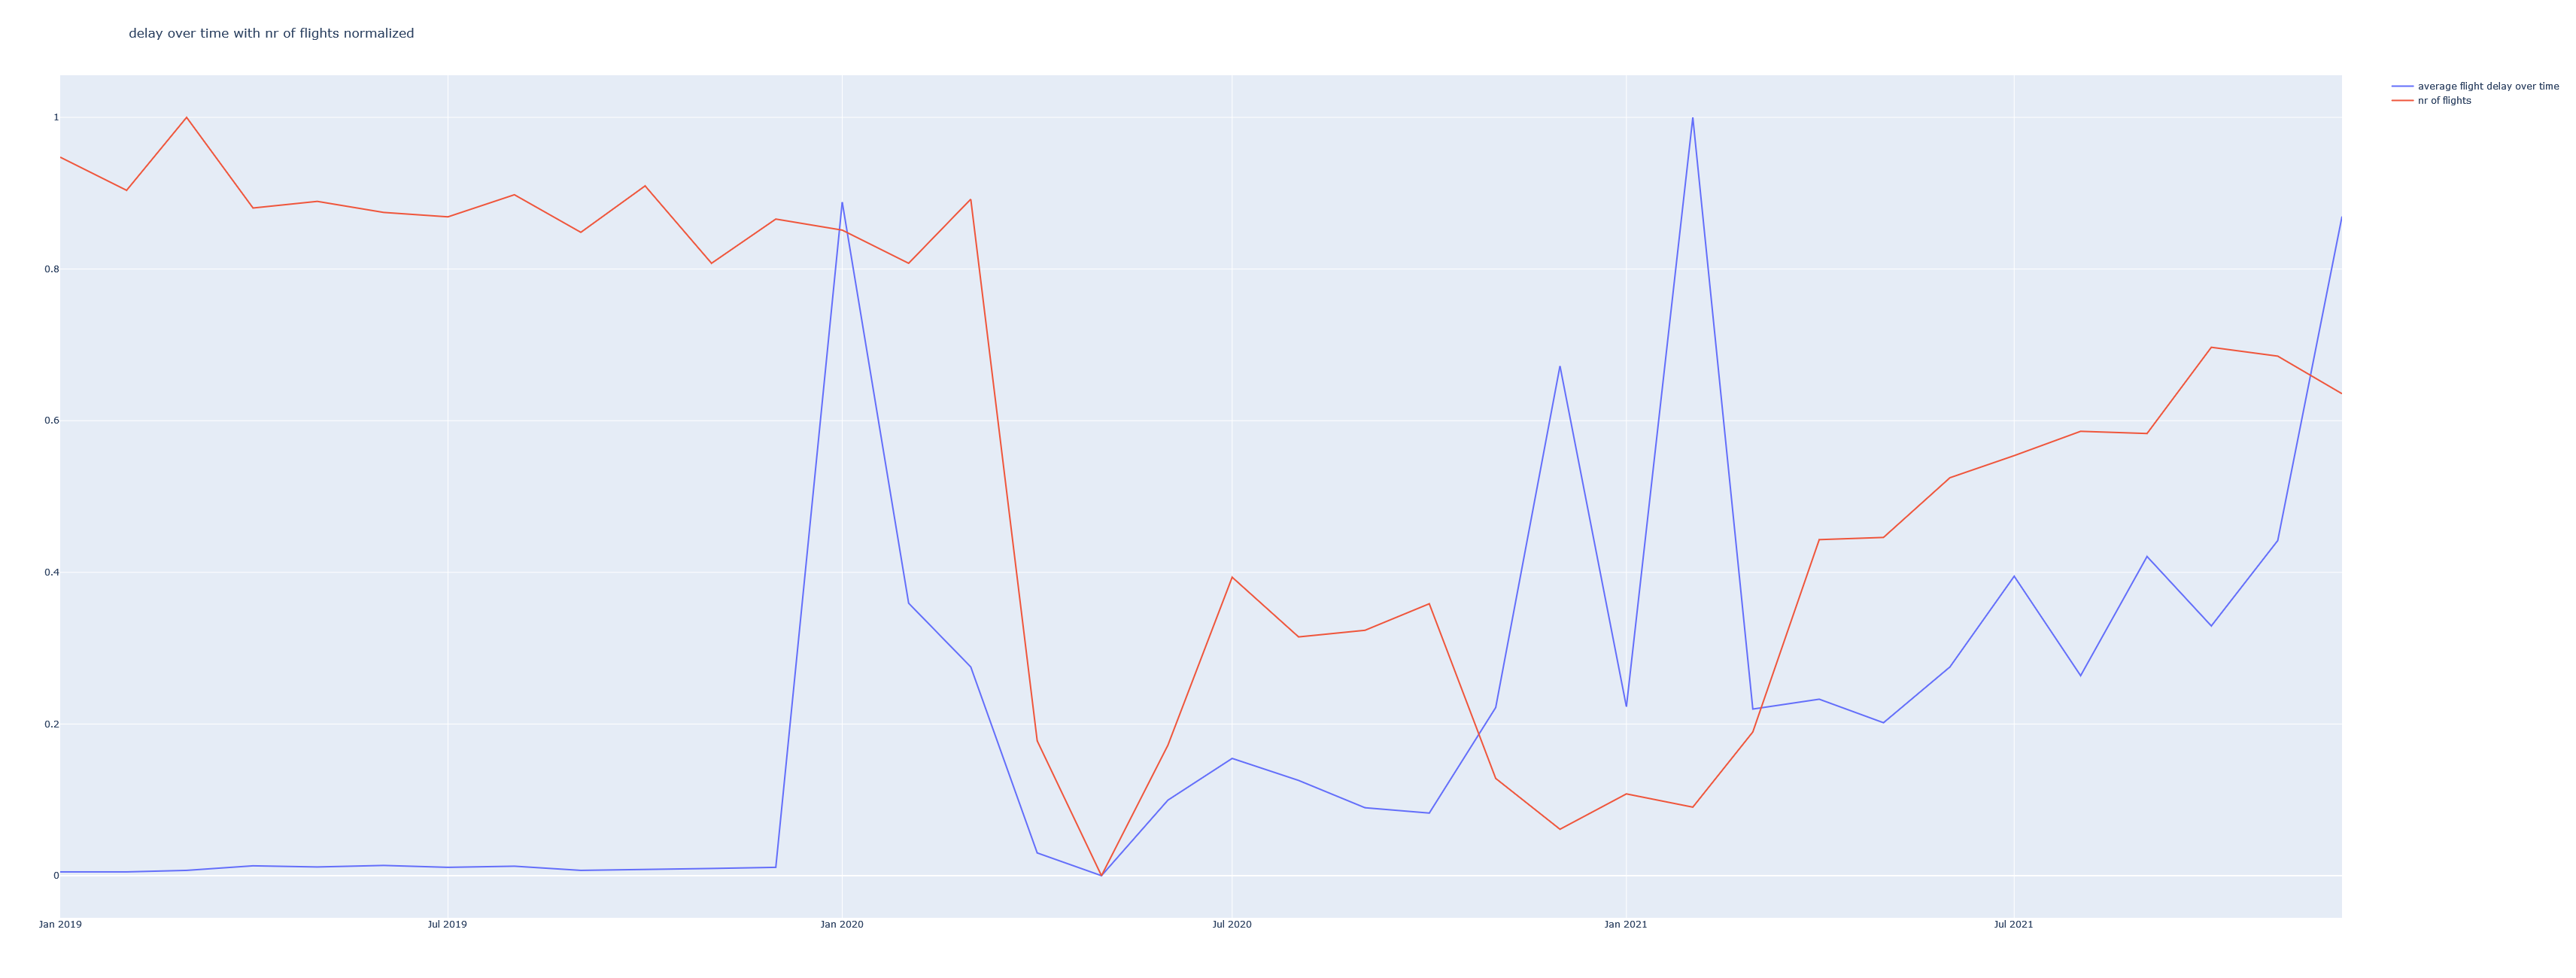
\includegraphics[width=11cm]{images/2019-2022.png}
    \label{fig:my_label}
\end{figure}
\end{frame}

\begin{frame}{A Graph! with a new year}
\begin{figure}
    \centering
    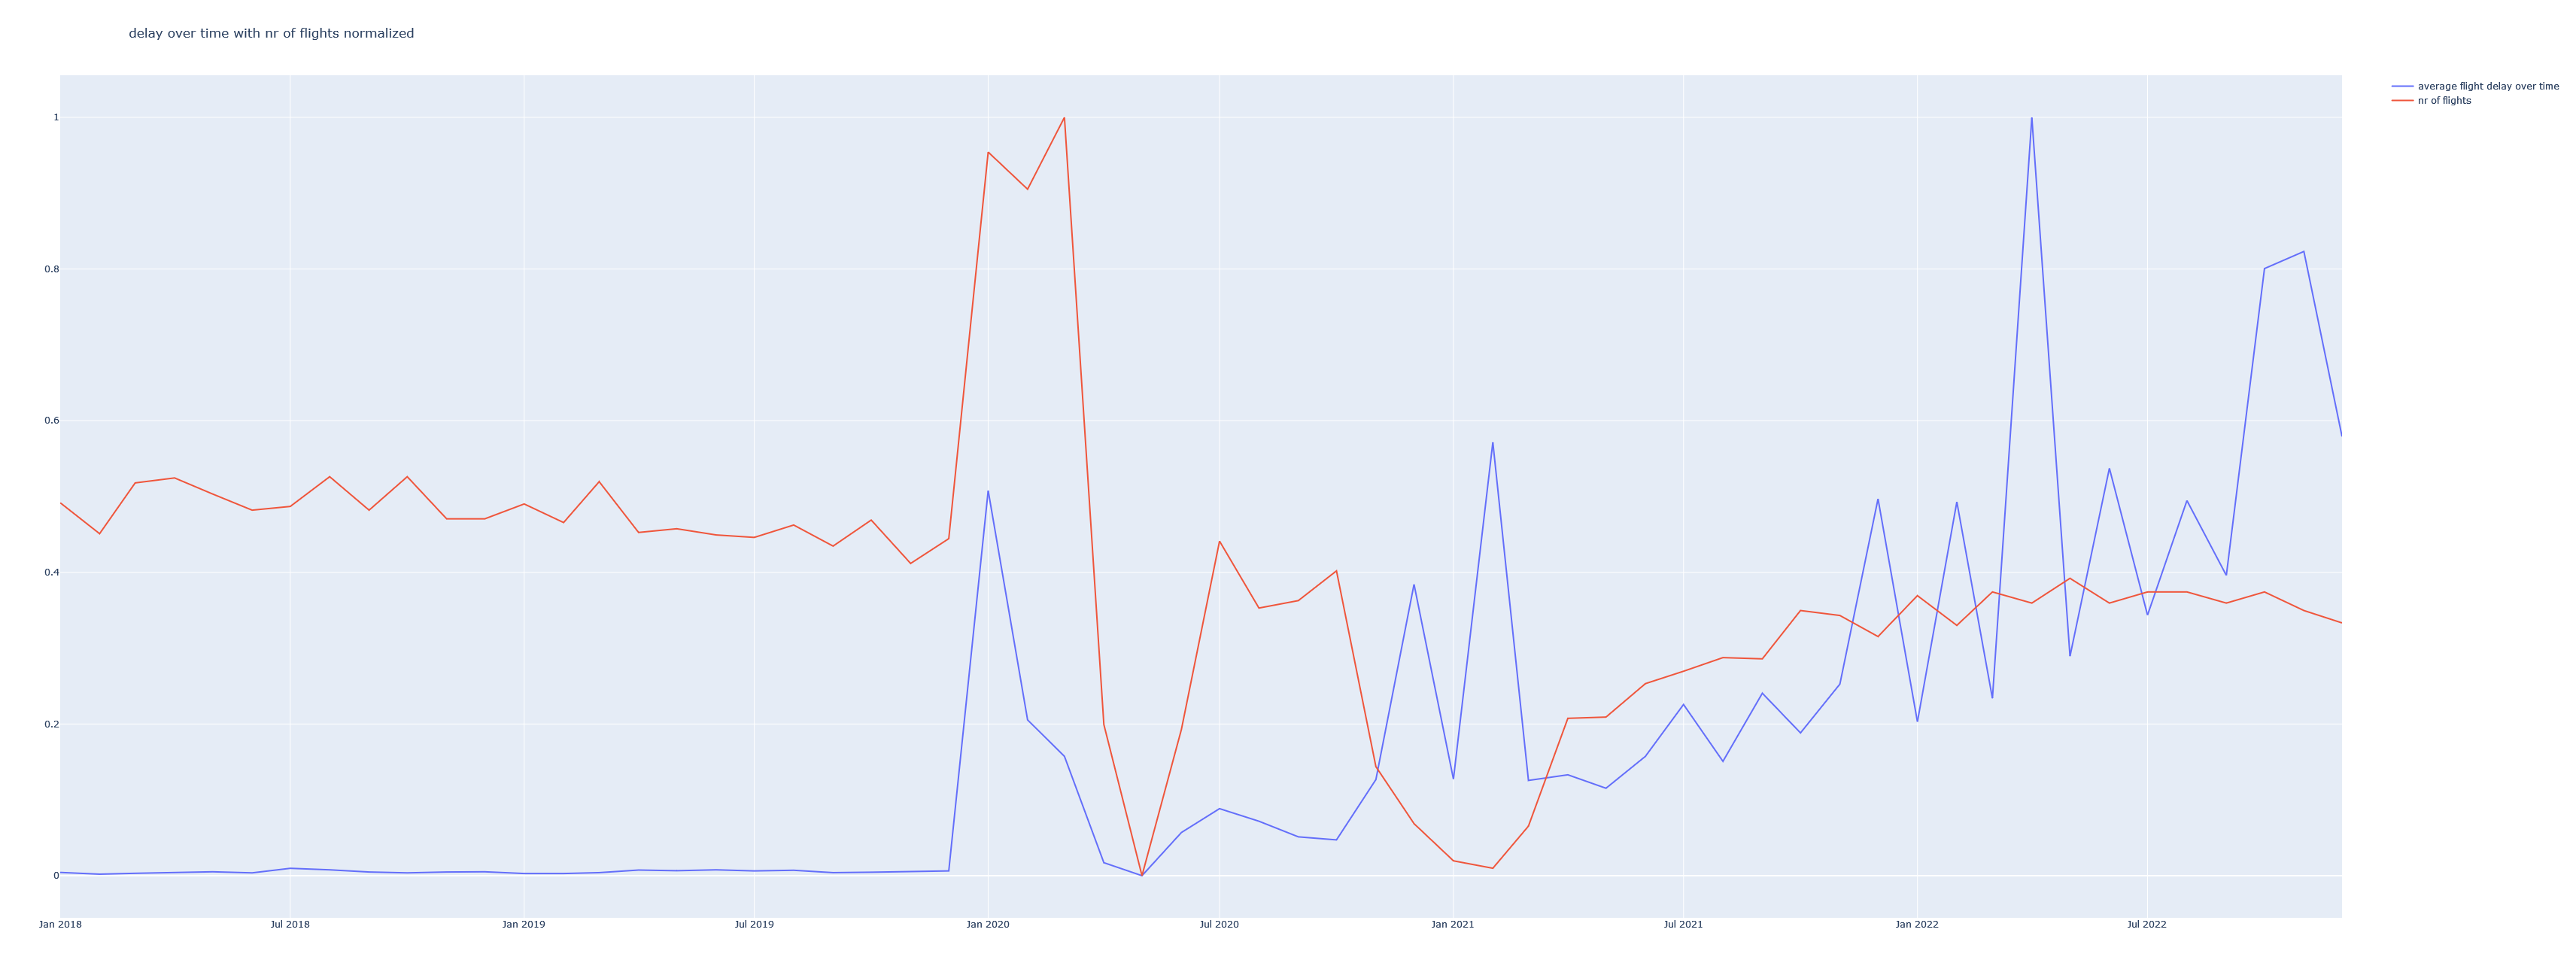
\includegraphics[width=11cm]{images/2018-2022.png}
    \label{fig:my_label}
\end{figure}
\end{frame}

\begin{frame}{A Graph! with bad information for 1 year}
\begin{figure}
    \centering
    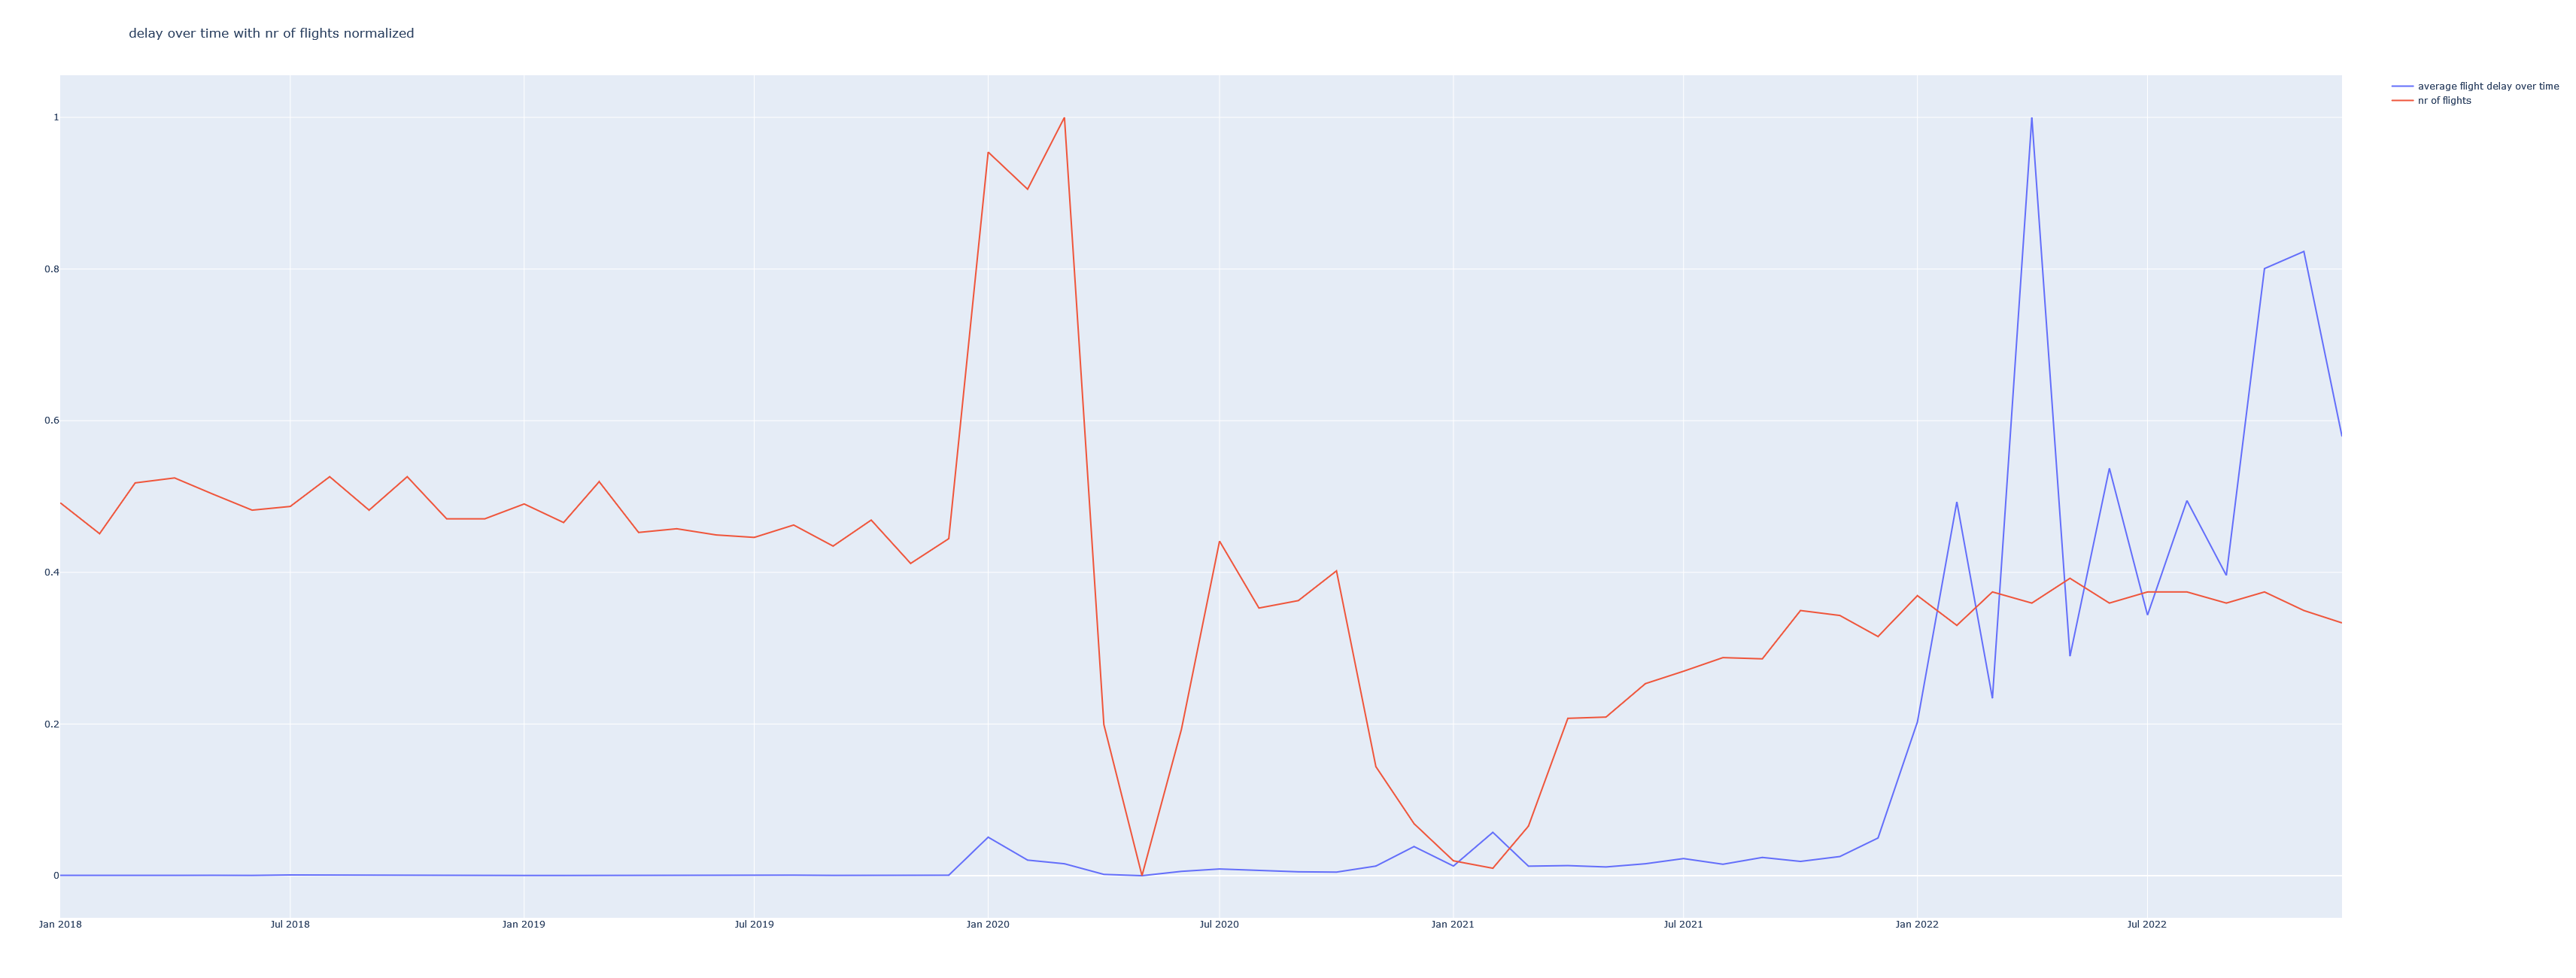
\includegraphics[width=11cm]{images/2018-2022bad.png}
    \label{fig:my_label}
\end{figure}
\end{frame}



%\appendix

%\begin{frame}[allowframebreaks]{References}

%  \bibliography{bibliography}
%  \bibliographystyle{abbrv}

%\end{frame}

\end{document}
